\chapter{Conception et Architecture du Système}
\label{ch:conception_architecture}

\section{Introduction}
Ce chapitre matérialise la traduction des concepts juridiques et réglementaires en composants logiciels concrets. Les choix architecturaux exposés ici sont justifiés par le prisme exclusif de la souveraineté numérique et de la sécurité des données, garantissant que l'infrastructure technique répond structurellement aux exigences des lois algériennes 18-07 et 25-11. Le système abandonne les approches déclaratives au profit d'une implémentation technique rigoureuse, où la conformité devient une propriété intrinsèque du code.

\section{Architecture Physique et Logique : Le Paradigme Souverain}
Le respect des impératifs légaux impose une dichotomie stricte dans la conception du système, séparant l'infrastructure d'hébergement de la logique applicative, tout en maintenant un contrôle absolu sur le cycle de vie de la donnée.

Le choix d'une architecture physique hébergée de manière strictement locale au sein d'un Datacenter \textit{On-Premise} constitue une obligation fonctionnelle non négociable. Cette topologie d'hébergement interdit techniquement et physiquement tout transfert de données à caractère personnel vers des juridictions étrangères, répondant ainsi expressément à l'interdiction de flux transfrontaliers stipulée par l'Article 44 de la loi 18-07. L'infrastructure réseau est isolée, interdisant toute connectivité sortante vers des fournisseurs Cloud internationaux, assurant une souveraineté de bout en bout.

D'un point de vue logiciel, l'architecture logique repose sur une conception modulaire et orientée microservices, segmentée en quatre blocs fonctionnels :
\begin{enumerate}
    \item \textbf{Frontend :} Interface utilisateur regroupant le portail web dédié à l'exploitation métier et le guichet DSAR public dédié à l'exercice des droits des personnes concernées.
    \item \textbf{Backend Métier \& IAM (\textit{Identity and Access Management}) :} Cœur transactionnel orchestrant le registre des traitements et la gestion centralisée des identités et des rôles via des jetons sécurisés (SSO/JWT).
    \item \textbf{Moteur d'Audit et Sécurité :} Composant cryptographique autonome imposant un algorithme de chiffrement asymétrique et symétrique de standard AES-256 au repos, couplé à une base de données de type WORM (\textit{Write Once Read Many}) garantissant la production de journaux de logs inaltérables.
    \item \textbf{Moteur IA Local :} Module d'intelligence artificielle générative encapsulé, déployant un LLM (\textit{Large Language Model}) totalement isolé du réseau public. Ce moteur exploite une architecture RAG (\textit{Retrieval-Augmented Generation}) pour interroger une base de données vectorielle contenant l'intégralité du corpus législatif algérien, sans recourir à des API externes, évitant ainsi toute fuite de données d'inférence.
\end{enumerate}

\section{Modélisation Statique : Diagramme de Classes \textit{Compliance by Design}}
L'ossature relationnelle de la base de données illustre la traduction de la législation en contraintes d'intégrité logicielle. Le modèle de données s'articule autour de trois blocs fondamentaux conditionnant le fonctionnement de la plateforme :

Le \textbf{Bloc IAM \& RBAC (\textit{Role-Based Access Control})} repose sur une entité abstraite \texttt{Utilisateur}, dont héritent les acteurs concrets \texttt{PersonneConcernee}, \texttt{DPO} et \texttt{EmployeMetier}. L'accès aux ressources est strictement encadré par des relations d'association avec les entités \texttt{Role} et \texttt{Permission}. Ce découplage garantit la ségrégation des privilèges et prévient l'escalade transactionnelle non autorisée.

Le \textbf{Bloc Gouvernance} structure la conformité opérationnelle. L'entité centrale \texttt{RegistreTraitement} est obligatoirement associée, par des contraintes de cardinalité strictes, aux entités \texttt{Finalite} (justifiant le "pourquoi" légitime du traitement), \texttt{Destinataire} (assurant la cartographie des flux imposée par l'Article 32 de la loi 18-07) et \texttt{CategorieDonnee}. Cette dernière entité porte un attribut booléen de sensibilité ou criticité, agissant comme un déclencheur conditionnel automatique pour les alertes de sécurité et l'activation de l'IA.

Le \textbf{Bloc Audit} matérialise l'imputabilité imposée par l'Article 41 bis 3 de la loi 25-11. L'entité critique \texttt{LogEvent} capte l'exhaustivité des interactions du système. Elle stocke formellement l'identifiant de l'auteur, l'action CRUD (\textit{Create, Read, Update, Delete}) exécutée, le système source, ainsi qu'un hash cryptographique généré en temps réel, conférant au journal général un état d'immuabilité mathématique.

\begin{figure}[H]
    \centering
    \includegraphics[width=\textwidth]{5-Chapters/Chapter3/DiagClass.png}
    \caption{Diagramme de Classes de la Plateforme (Compliance by Design)}
    \label{fig:dc_chapter3}
\end{figure}

\section{Modélisation Dynamique : Flux Critiques}
La dynamique d'exécution de la plateforme démontre physiquement la robustesse du système face aux vecteurs de compromission. Les processus métiers illustrent les mécanismes de validation interceptant inéluctablement les requêtes.

\textbf{Processus 1 : Consultation sécurisée d'une donnée chiffrée.}
La consultation d'une information sensible obéit à une chaîne d'autorisation stricte. Lorsqu'un \texttt{EmployeMetier} initie une requête de lecture depuis le Frontend, le Backend intercepte l'appel et réalise une vérification algorithmique de la signature du jeton JWT. Si l'identité est confirmée, le système exige dynamiquement la fourniture d'un motif d'accès textuel. Une fois ce motif validé, le Moteur Crypto procède au déchiffrement de la donnée, chiffrée en AES-256, survenant exclusivement en mémoire vive (RAM). Simultanément, avant la transmission de la réponse HTTP vers le client, un enregistrement \texttt{LogEvent} infalsifiable est généré vers la base WORM. L'affichage en clair de la donnée n'intervient qu'une fois la preuve d'audit cryptographiquement validée et scellée.

\textbf{Processus 2 : Réalisation d'une AIPD (Étude d'Impact) avec l'IA Souveraine.}
Lorsqu'un traitement réclame une vigilance particulière, le DPO engage une Étude d'Impact (AIPD) assistée par l'IA. Ce processus s'amorce par la soumission, via l'interface métier du DPO, des métadonnées caractérisant le traitement. La requête est acheminée vers le Moteur IA Local, instanciant un agent autonome LLM. Ce dernier interroge dynamiquement sa base vectorielle (RAG) sur la jurisprudence locale et les textes de loi applicables. L'agent IA détecte analytiquement des marqueurs de risque critiques, tel que la présence inhérente de biométrie dans le jeu de données. Sur la base de cette inférence, le moteur évalue algorithmiquement un score de risque résiduel unitaire, et génère de façon autonome un rapport structuré de recommandations juridiques, sans qu'aucune portion des données de traitement ne franchisse le périmètre de l'infrastructure locale.

\begin{figure}[H]
    \centering
    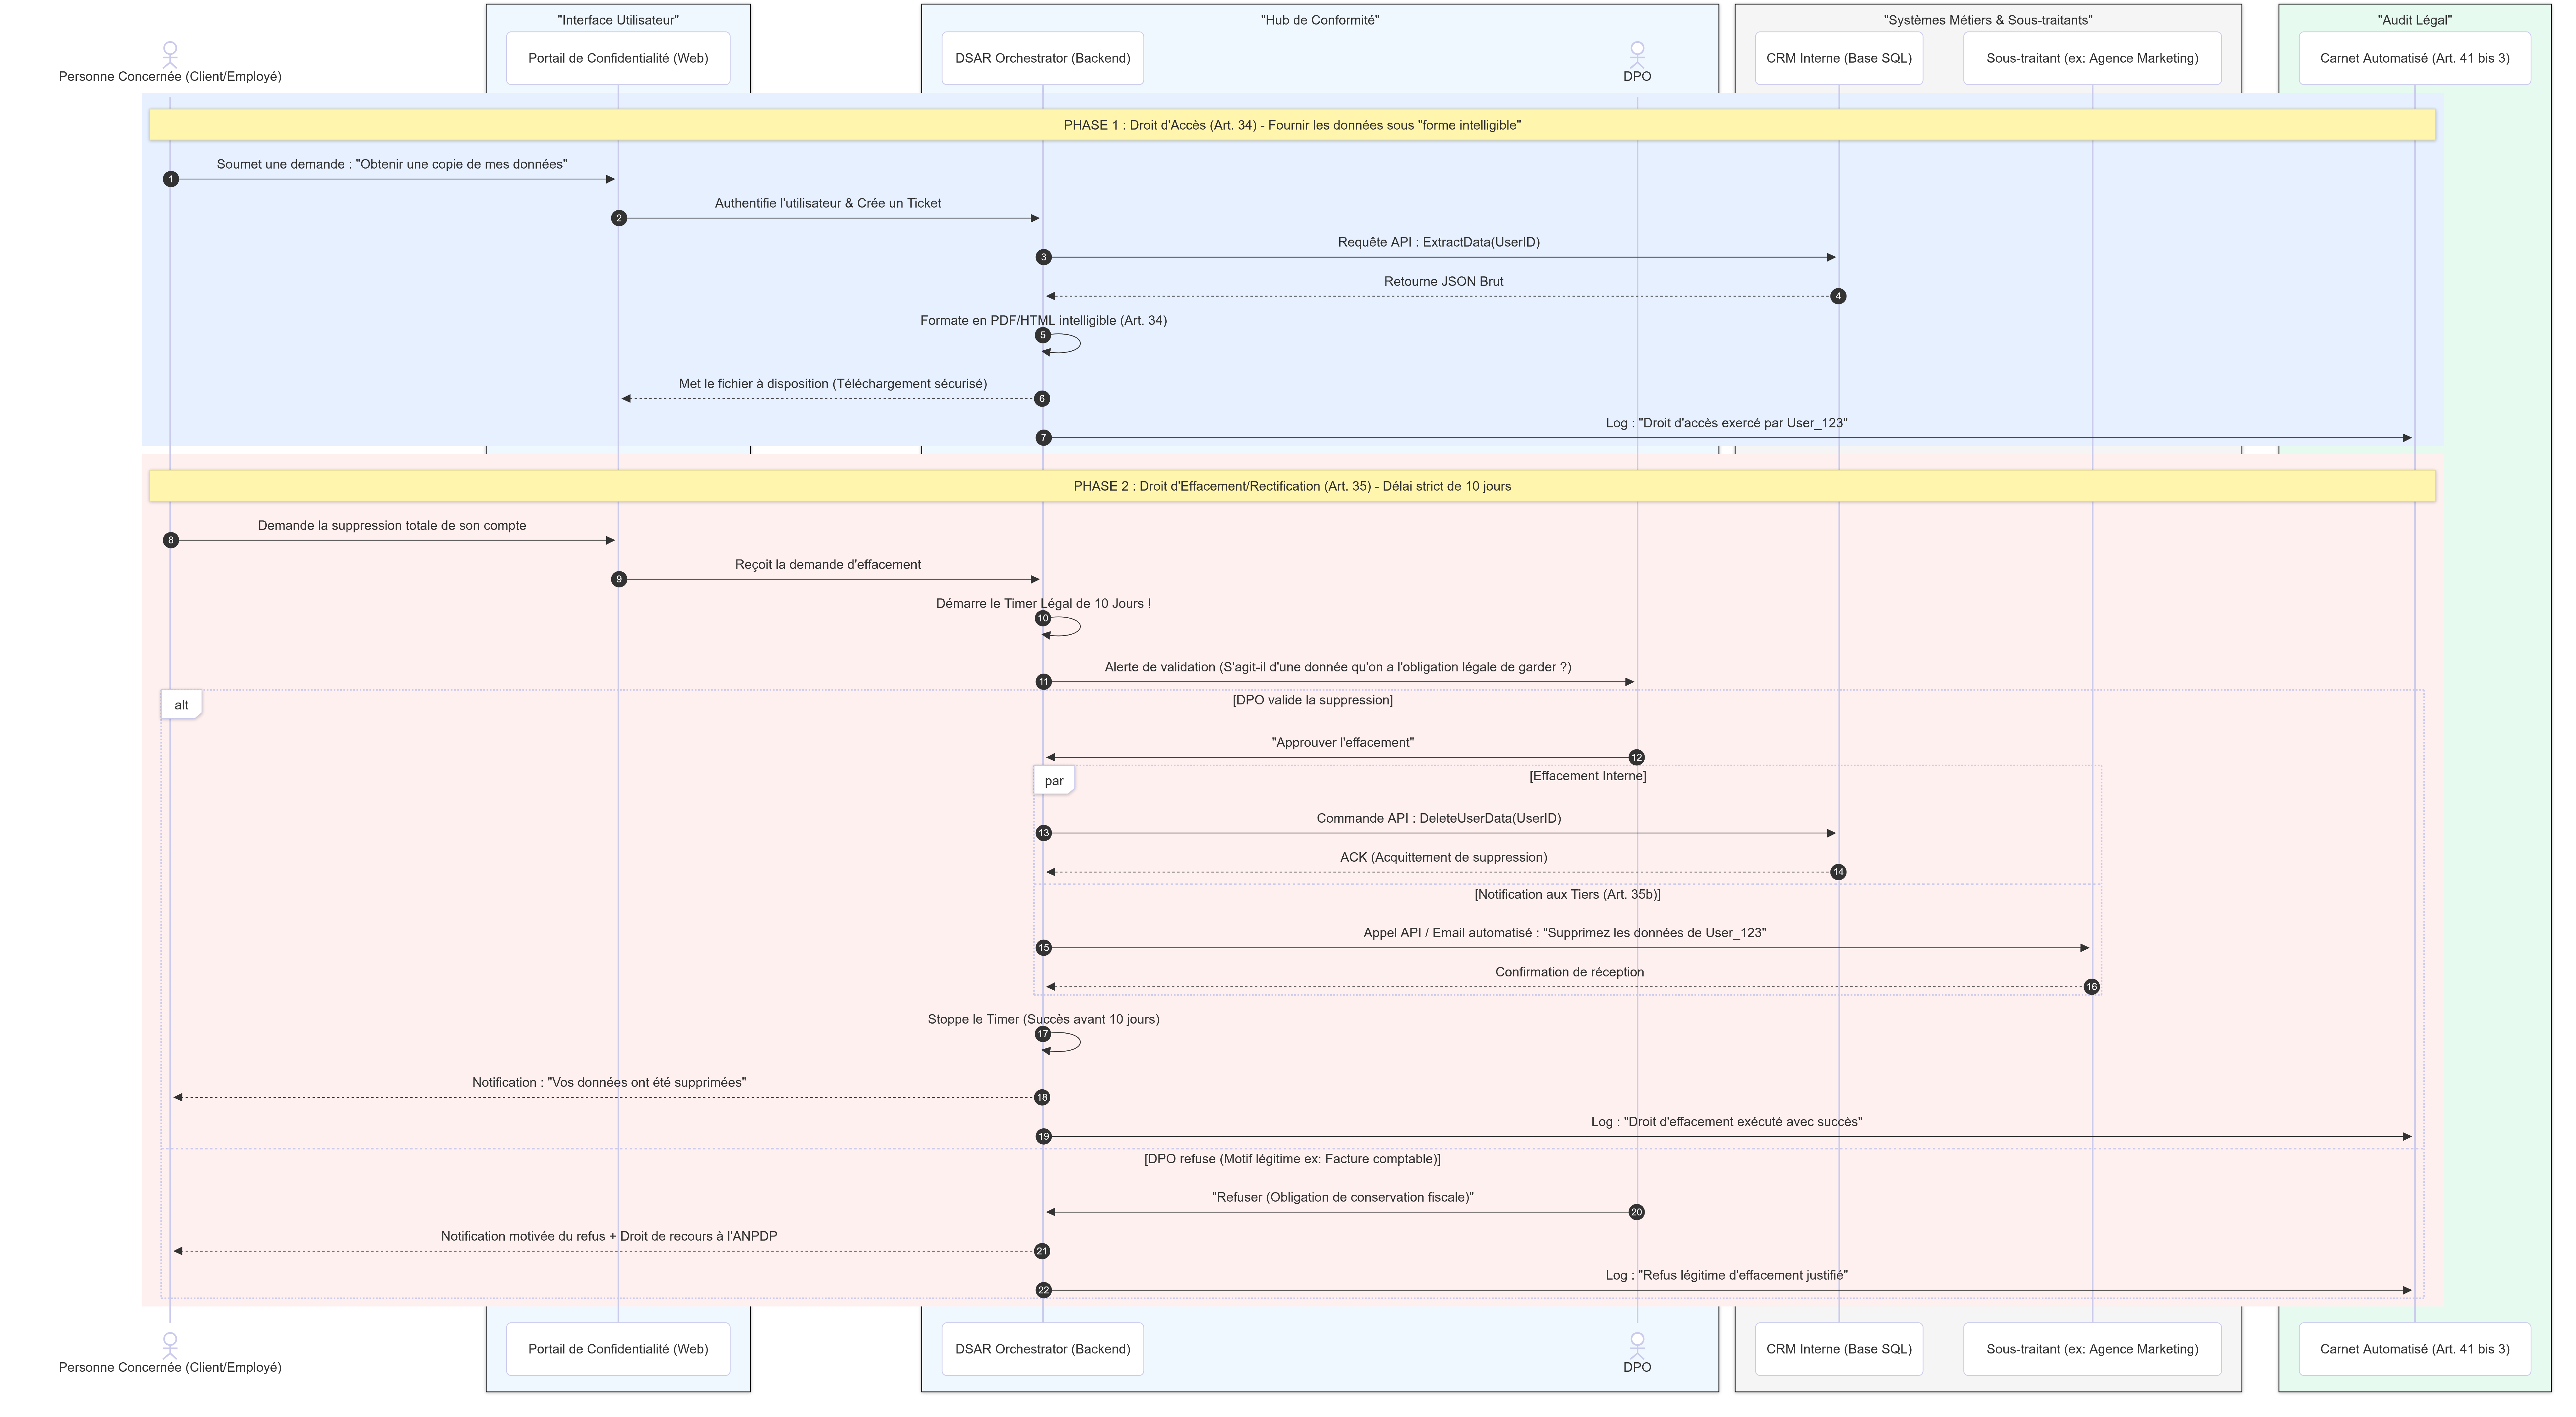
\includegraphics[width=\textwidth]{5-Chapters/Chapter3/DS_DroitPerson.png}
    \caption{Diagramme de Séquence : Flux Critiques}
    \label{fig:ds_droitperson}
\end{figure}

\section{Conclusion}
L'architecture logicielle modélisée au sein de cette plateforme démontre que la souveraineté et la cybersécurité ne relèvent pas uniquement de dispositions déclaratives, mais exigent une ingénierie logicielle coercitive et mesurable. Par la conjonction d'une infrastructure \textit{On-Premise}, d'un audit immuable au format WORM et d'un contrôle d'accès cryptographique, ce chapitre acte une transition majeure : la conformité légale (Lois 18-07 et 25-11) s'émancipe de la procédure humaine potentiellement faillible pour devenir un processus mathématique, déterministe et algorithmique intégré nativement au compilateur et à l'exécution de l'application, instituant définitivement le principe de \textit{Compliance by Code}.
